\chapter{Cơ sở lý thuyết và công nghệ sử dụng}

\section{Giải pháp quản lý phân phối}
\subsection{Các khái niệm trong quản lý phân phối}
Trước tiên, ta cần tìm biết về một từ khóa đã trở nên rất
phổ biến trong thời gian gần đây, đó là Logistics. Hiểu một cách đơn
giản thì Logistics là quá trình lên kế hoạch, áp dụng và kiểm soát
các luồng dịch chuyển của hàng hóa hay thông tin liên quan tới nguyên
nhiên liệu vật tư (đầu vào) và sản phẩm cuối cùng (đầu ra) từ thời
điểm xuất phát tới điểm tiêu thụ. Đi kèm với Logistics là khái niệm
về Quản trị chuỗi cung ứng (Supply Chain Management), Quản trị chuỗi
cung ứng bao gồm tất cả những hoạt động quản trị logistics cũng như
những hoạt động sản xuất và thúc đẩy sự phối hợp về quy trình và
hoạt động của các bộ phận marketing, kinh doanh, thiết kế sản phẩm,
tài chính, công nghệ thông tin. Khái niệm chuỗi cung ứng rộng hơn,
bao gồm cả logistics và quá trình sản xuất. Ngoài ra chuỗi cung ứng
chú trọng hơn đến hoạt động mua hàng (procedurement) trong khi
logistics giải quyết các vấn đề chiến lược, phối hợp giữa marketing và
sản xuất.

Khi đã có một hình dung cơ bản về chuỗi cung ứng, ta đến với
phần chính là \textbf{hệ thống quản lý phân phối}
(Distribution Management System). Hệ thống quản lý phân phối
(Distribution Management System) là phần mềm quản lý chuỗi
cung ứng hàng hóa của doanh nghiệp, giúp họ quản lý các hoạt
động phân phối hàng hóa ra thị trường, kiểm soát các kênh phân
phối, quản lý nhân viên, người bán hàng, kiểm soát hàng hóa
trong kho, hàng tồn kho, kế hoạch vận chuyển
hàng hóa đến địa chỉ mua hàng,…

Ví dụ, Masan Group là một công ty lớn trong lĩnh vực kinh tế
tư nhân Việt Nam, tập trung hoạt động trong ngành hàng tiêu dùng và
tài nguyên của Việt Nam. Masan quản lý các nền tảng kinh doanh có
quy mô lớn nhằm phát triển và khai thác các tiềm năng trong lĩnh vực
tiêu dùng và tài nguyên. Còn rất nhiều những tập đoàn bán lẻ khác
có cùng cơ chế quản lý kinh doanh như Masan, mỗi tập đoàn như vậy đều
cần có một hệ thống riêng để quản lý chuỗi cung ứng của mình.

Vì vậy Distribution Management System là một trong số những
phần mềm quản lý doanh nghiệp có tính ứng dụng cao, phù hợp với mọi
doanh nghiệp sản xuất và phân phối. Đối với các doanh nghiệp lớn
(ví dụ Masan, VinGroup) có đội ngũ nhân viên bán hàng đông đảo và các
kênh phân phối phức tạp, phần mềm DMS càng quan trọng và là công cụ không
thể thiếu. Các nhà quản lý của các tập đoàn lớn này luôn đau đầu vì
những câu hỏi như “Làm thế nào để nắm được nhanh nhất xu thế, biến động
của thị trường?”, “Làm thế nào để kiểm soát phân phối tốt, duy
trì tồn kho ở mức tối ưu, tiết kiệm thời gian?”, “Tự động hóa bán
hàng, tăng hiệu quả bán hàng cho đội ngũ nhân viên bán hàng như
thế nào?”. Với hệ thống quản lý kênh phân phối (DMS), các doanh nghiệp
lớn với vài trăm, hoặc vài nghìn nhân viên bán hàng, hàng chục
nghìn điểm bán sẽ dễ dàng làm được việc này.

\subsection{Lợi ích của hệ thống quản lý phân phối}
Phần trên đã trình bày về lý do tại sao các doanh nghiệp và tập
đoàn bán lẻ phải sử dụng giải pháp quản lý phân phối và sau đây
là những lợi ích chính, thấy rõ nhất theo như tìm hiểu của em.

Thứ nhất Distribution Management System là công cụ tự động hóa
bán hàng, giúp nhân viên bán hàng (salesman) tiết kiệm thời gian,
tăng chất lượng chăm sóc khách hàng, tối ưu doanh thu. Mọi thông
tin nhân viên bán hàng cần khi ghé thăm một điểm bán lẻ (rental outlet) 
bao gồm thông tin về khách hàng (customer), lịch sử mua hàng, 
các báo cáo bán hàng, thông tin sản phẩm, chương trình khuyến mãi,… 
có sẵn trong ứng dụng di động DMS để nhân viên có thể dễ dàng theo
dõi tại điểm bán.

Thứ hai Distribution Management System có thể quản lý hiệu quả
làm việc của nhân viên bán hàng, nhà quản lý có thể nắm được lộ
trình ghé thăm khách hàng của nhân viên trên bản đồ lịch sử checkin.
Thông qua đó đánh giá được nhân viên bán hàng có đang tích cực
ngoài thị trường hay không, khách hàng có được chăm sóc tốt hay không.

Thứ ba, đặc biệt hơn là qua hệ thống nhà quản trị sẽ biết
được những cửa hàng nào đang liên tục phát sinh doanh số, những cửa hàng
nào lâu rồi chưa phát sinh đơn hàng mới. Từ đó có thể sắp xếp,
phân chia hợp lý các nhân viên bán hàng vào các tuyến bán
hàng, thay đổi tần suất viếng thăm khách hàng cho phù hợp với
thực tế, tránh lãng phí nguồn lực đồng thời có thể chăm sóc được kỹ
hơn các cửa hàng trọng tâm.

Thứ tư, cập nhật thị trường là điểm nổi bật của phần mềm 
Distribution Management System. Giúp các doanh nghiệp phân phối có thể
kiểm soát được hàng tồn tại từng điểm bán lẻ, đại lý nhằm
đưa ra kế hoạch sản xuất, điều phối hàng hóa phù hợp.

\subsection{Khảo sát thực tế việc sử dụng hệ thống quản lý phân phối}
Khi chưa sử dụng Distribution Management System, có rất nhiều
lỗ hổng mà các doanh nghiệp phân phối phải đối mặt như sau đây:
\begin{itemize}[topsep=0ex]
\item Hàng tồn kho: Không kiểm soát được hàng tồn kho của nhà
    phân phối, cửa hàng để tối ưu hóa chuỗi cung ứng và các
    chiến lược tiêu thụ hàng. Công ty sẽ không có sự chủ động trong
    việc cung ứng và tiêu thụ hàng trên thị trường, đặc biết là loại
    mặt hàng có thời hạn sử dụng ngắn, sẽ không kiểm soát được hàng
    đang ở đâu trong chuỗi cung ứng của mình.

\item Bao phủ: Việc quản lý và tối ưu tuyến bán hàng theo từng
    ngành hàng, khu vực, đội bán hàng để gia tăng độ bao phủ
    cũng là một vấn đề.

\item Doanh số: Doanh số luôn là vấn đề đau đầu của các nhà quản lý,
    họ sẽ không có đầy đủ thông tin để triển khai các chương trình
    bán hàng một cách có hiệu quả.

\item Hiệu suất: Làm thế nào để biết đội ngũ bán hàng của công ty
    có hoạt động với hiệu suất 100\% hoặc hơn không? Làm sao để
    thiết kế các KPI và kiểm soát hiệu quả giúp họ có động lực bán
    hàng, tăng hiệu suất làm việc? Đội ngũ nhân viên bán hàng có
    được theo sát và huấn luyện các kỹ năng bán hàng hay không?

\item Số ảo: Tình trạng số ảo khá phổ biến trong bán hàng và phân phối,
    các số liệu ảo về điểm bán, doanh số, khuyến mãi, tồn kho, …
    luôn là nỗi lo lắng của các nhà quản lý vì điều này ảnh hưởng lớn
    đến việc ra quyết định của họ.

\item Tích hợp: Trong mô hình phân phối hiện đại và đa kênh, các công
    ty cung cấp, phân phối hàng hóa ra thị trường cũng sẽ đối diện
    với vấn đề tiếp xúc và xử lý thông tin với nhiều hệ thống, hình
    thức dữ liệu khác nhau. Làm thế nào để thiết kế mô hình dữ liệu
    chung đồng nhất nhưng vẫn đảm bảo các quy trình, điểm đặc thù
    của mỗi kênh, mỗi hệ thống, đảm bảo tính xuyên suốt, đồng nhất
    và kịp thời của thông tin.
\end{itemize}

Còn sau khi áp dụng giải pháp quản lý hệ thống phân phối
(DMS) thì các nhà quản lý thu được:
\begin{itemize}[topsep=0ex]
\item Dữ liệu thật: Với các quy trình và chức năng được thiết kế chặt
    chẽ và hỗ trợ hiệu quả các đối tượng sử dụng trong hệ thống sẽ
    giúp công ty có được bộ dữ liệu đầy đủ và thật từ dữ liệu
    thị trường, điểm bán, tuyến bán hàng đến tồn kho, sell-in, sell-out,
    khuyến mãi, trưng bày, … hạn chế và ngăn chặn tối đa các trường hợp
    thay đổi dữ liệu bán hàng. Dữ liệu thất này sẽ giúp công ty ra
    quyết định và triển khai các chiến lược bán hàng hiệu quả
    và chính xác hơn.

\item Chủ động và làm chủ thị trường: Doanh nghiệp hoàn toàn chủ động
    trong triển khai chiến lược bán hàng, chủ động khi có sự thay đổi,
    biến động về nhân sự trong hệ thống phân phối và dễ dàng thiết
    lập các nhà phân phối mới, khu vực mới cho các hệ thống bán hàng mới.

\item Gia tăng giá trị thương hiệu: Việc triển khai và quản lý hiệu
    quả các chương trình bán hàng giúp thu hút và thúc đẩy tiêu thụ
    từ người tiêu dùng làm gia tăng sự trung thành từ người tiêu
    dùng cũng như sự hợp tác từ nhà phân phối vì
    họ thấy được lợi ích thật sự
\end{itemize}

Hiện nay trên thị trường có một số ít sản phẩm phần mềm quản lý hệ
thống phân phối cho doanh nghiệp (DMS). Sử dụng phần mềm này thường
là những người quản lý của doanh nghiệp, công ty, hãng phân phối.
Do tính chất đặc thù như vậy mà những người tiếp cận và sử dụng phần
mềm kiểu này này khá ít, và phần mềm quản lý hệ thống phân phối DMS
cũng không phổ biến rộng rãi cho mọi đối tượng. Một số phần mềm DMS
có thể kể đến như Adaline, BS Silver, SSE, Perfect Warehouse, GM Sales,
KiotViet, Suno, Sapo, … Mỗi phần mềm sẽ cung cấp những tính năng đặc
biết riêng, tính phí hoặc không tính phí, dùng offline hoặc online, từng
nền tảng (Windows, Android, iOS) và ưu nhược điểm khác nhau. Các phần
mềm offline như Adaline, BS Silver, Perfect Warehouse, … sẽ có ưu điểm
là miễn phí, tốc độ nhanh, bảo mật cao. Tuy nhiên chỉ phù hợp với những
cửa hàng bán lẻ, vừa và nhỏ, tính năng hạn chế, không có khả năng mở
rộng. Sapo hay KiotViet là các phần mềm quản lý phân phối phổ biến
hơn khi cung cấp cho người dùng nhiều tính năng với mức giá rẻ, giao
diện làm việc trực tuyến, nhanh, dễ sử dụng, … Các phần mềm kiểu này
phù hợp với những công ty, doanh nghiệp phân phối lớn hơn khi khả năng
nắm bắt biến động thị trường là cần thiết để đưa ra những
chiến lược kinh doanh kịp thời.

Ở Việt Nam hiện nay, KiotViet là phần mềm quản lý bán hàng phổ biến
nhất với hơn 100,000 cửa hàng đang sử dụng và hơn 5,000 cửa hàng mới
mỗi tháng. Đơn giản, dễ dùng, tiết kiệm chi phí và phù hợp với hơn
15 ngành hàng khác nhau. KiotViet sẽ cung cấp cho người dùng một khung
tính năng cố định ứng với từng ngành hàng khác nhau. Một phần mềm
quản lý hoàn chỉnh có hai phần, một là trang quản lý, hai là trang
bán hàng. Trang quản lý của KiotViet có các tính năng về quản lý hàng
hóa (quản lý danh mục, thiết lập giá, …), quản lý giao dịch (lên hóa đơn,
đặt hàng, xuất hàng, …), quản lý nhân viên, quản lý khách hàng và
nhà cung cấp, xuất báo cáo (cuối ngày, theo tuần, theo tháng ,…).
Trang bán hàng của KiotViet cung cấp một giao diện đơn giản tương tự
như giao diện thanh toán bán hàng ở các cửa hàng bán lẻ hay
siêu thị nhỏ. Đơn giản chỉ chọn sản phẩm, tính tiền, thanh toán
và xuất hóa đơn cho khách.

Trong ứng dụng quản lý phân phối của chúng em, ngoài những tính
năng cơ bản, cần thiết như quản lý sản phẩm, quản lý hàng trong kho,
quản lý giao dịch, quản lý nhân viên, quản lý phân quyền động thì ứng
dụng một tính năng mới. Đó là ứng dụng cung cấp chức năng gợi ý,
lên lịch trình viếng thăm cho các nhân viên bán hàng (salesman), lưu
lại lịch sử check-in của nhân viên bán hàng. Nhân viên bán hàng
là người hàng ngày sẽ thăm một số cửa hàng bán lẻ (rental outlet),
kiểm tra lượng hàng hóa bán ra, từ đó lên hóa đơn để nhập hàng hóa
mới về. Để các nhân viên bán hàng này hoạt động hiệu quả nhất, cần
phân công họ vào các tuyến bán hàng phù hợp, để họ vừa có thể di chuyển
một cách dễ dàng giữa các cửa hàng bán lẻ, vừa đến được nhiều cửa
hàng nhất có thể. Chi tiết về tính năng mới này sẽ được trình bày
trong chương sau của đồ án.

\section{Cơ sở lý thuyết}
\subsection{Role-Based Access Control}
Trong an toàn thông tin, role-based access control (RBAC) là
một cách tiệp cận cho vấn đề hạn chế quyền truy cập của
người dùng. RBAC được sử dụng phổ biến tại các tổ chức
lớn với nhiều hơn 500 nhân viên. 

RBAC có nhiều mô hình khác nhau. Mô hình cơ bản là
$\text{RBAC}_0$, mô hình có chứa quan hệ phân cấp là
$\text{RBAC}_1$, có chứa ràng buộc $\text{RBAC}_2$ và mô hình tăng
cường (consolidated) $\text{RBAC}_3$.

Các thành phần chính của RBAC bao gồm user (người dùng),
role (vai trò), permission (quyền) và session (phiên truy cập)
cùng với quan hệ giữa chúng nhằm đơn giản hóa quá trình
gán quyền cho người dùng. 

User hay người dùng trong mô hình RBAC là con người, tuy nhiên
khái niệp này có thể được tổng quát hóa bằng việc bao gồm cả những
tác nhân tự động như robot hay phần mềm khác. Một role là một
chức năng công việc hay chức vụ trong tổ chức đi kèm với các
thẩm quyển mà nhân viên trong chức vụ đó nắm giữ. Còn một
permission là sự một chấp nhận cho một phương thức truy cập
vào một hay nhiều các đối tượng trong hệ thống. Việc một
permission tương ứng với gì thì tùy thuộc vào hệ thống
implement ra sao mô hình RBAC.

Mỗi một session là một ánh xạ từ mỗi phần tử của tập user
sang tập con của tập các role. Session thiết lập một phiên
truy cập với tập các role được kích hoạt (là một tập con
của tập các role mà người dùng đó được gán). Mỗi một phiên truy
cập tương ứng cho một user, trong $\text{RBAC}_0$ sự tương ứng này
là không thay đổi theo thời gian.

Trong RBAC, permission được gán với một hoặc nhiều role,
người dùng hay nhân viên được gán với một hay nhiều role.
Người dùng trong RBAC không được gán trực tiếp các permission mà
phải thông qua role, từ đó đơn giản hóa quá trình gán
permission hay việc chuyển phòng ban công tác của nhân viên. 

Trong đồ án này chỉ sử dụng mô hình điều khiển truy cập
dựa trên $\text{RBAC}_0$, biểu diễn toán học của $\text{RBAC}_0$ như sau:
\begin{itemize}[topsep=0ex]
\item Tập $U$, $R$, $P$ và $S$ tương ứng với tập hợp của các
    user, role, permission và session.
\item Tập $PA \subseteq P \times R$ biểu diễn quan hệ nhiều nhiều
    giữa permission và role.
\item Tập $UA \subseteq U \times R$ biểu diễn quan hệ nhiều nhiều giữa user và role.
\item Ánh xạ $user: S \rightarrow U$ gán mỗi một
    session $s$ cho một user $user(s)$.
\item Ánh xạ $roles: S \rightarrow \mathcal{P}(R)$ gán mỗi một
    session $s$ cho tập con của các role: 
    $roles(s) \subseteq \{ r | \left( user(s), r \right) \in UA \}$
    (có thể thay đổi theo thời gian) và session sẽ có các permission
    là $\bigcup_{r \in roles(s)}  \{ p | (p, r) \in PA \}$
\end{itemize}

\begin{figure}[H]
\centering
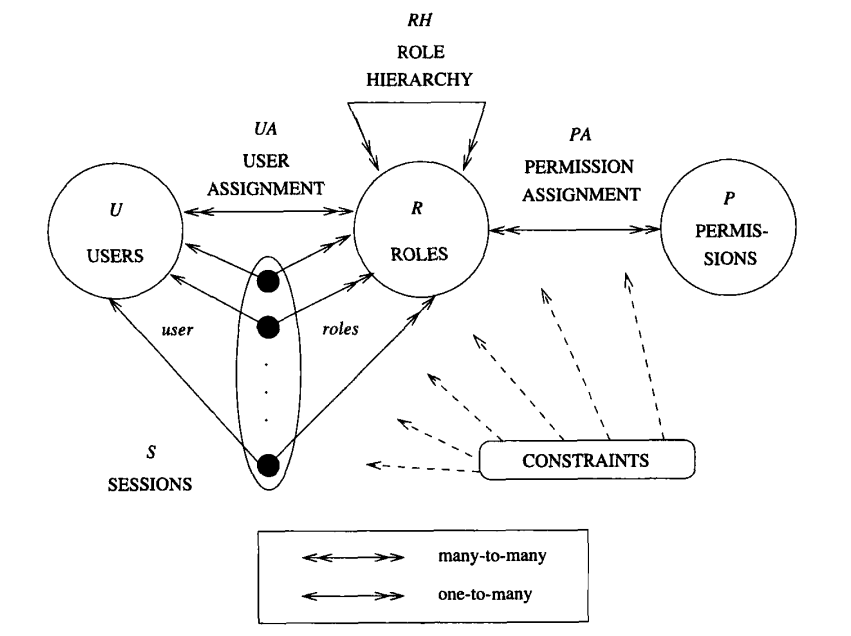
\includegraphics[width=12cm]{images/RBAC.png}
\caption{Các mô hình RBAC}
\end{figure}

\subsection{Thuật toán phân cụm dữ liệu}
\subsubsection{Giới thiệu về bài toán phân cụm dữ liệu}
Phân cụm là kỹ thuật quan trọng trong xử lý dữ liệu, nó thuộc lớp
các phương pháp học không giám sát (Unsupervised Learning) trong học
máy (Machine Learning). Giải thích dễ hiểu hơn thì phân cụm là
các quy trình tìm cách nhóm các đối tượng đã cho vào các cụm (cluster),
sao cho các đối tượng trong cùng một cụm tương tự nhau (similar) và
các đối tượng khác cụm thì không tương tự nhau (dissimilar).

Mục đích của phân cụm là tìm ra bản chất bên trong các
nhóm của dữ liệu và có thể  áp dụng trong rất nhiều lĩnh vực như:
\begin{itemize}[topsep=0ex]
\item Trong marketing, xác định các nhóm khách hàng (khách hàng tiềm
    năng, khách hàng giá trị, phân loại và dự đoán hành vi khách
    hàng, …) sử dụng sản phẩm hay dịch vụ của công ty để giúp
    công ty có chiến lược kinh doanh hiệu quả hơn.

\item Trong sinh học, phân nhóm động vật và thực vật
    dựa vào các thuộc tính của chúng.

\item  Trong bảo hiểm, tài chính: phân nhóm các đối tượng
    sử dụng bảo hiểm và các dịch vụ tài chính, dự đoán xu hướng
    của khách hàng, phát hiện gian lận tài chính, …

\item Trong phân tích dữ liệu web: phân loại tài liệu, phân
    loại người dùng web, …
\end{itemize}

\subsubsection{Thuật toán K-Means}
K-Means là thuật toán quan trọng và được sử dụng phổ biến
trong kỹ thuật phân cụm. Tư tưởng chính của thuật toán K-Means
là tìm cách phân nhóm các đối tượng đã cho vào $K$ cụm ($K$ là
số cụm được xác định trước, $K$ nguyên dương) sao cho khoảng các từ
các đối tượng đến tâm nhóm (centroid) là nhỏ nhất.

Phát biểu bài toán: Cho $N$ điểm trên không gian $d$ chiều.
Làm thế nào để phân chia thành $K$ nhóm mà các điểm trong
một nhóm có khoảng cách gần trọng tâm của nhóm hơn so với
khoảng cách đến trọng tâm của bất kì 1 nhóm nào khác.

Đầu vào, đầu ra của thuật toán:
\begin{itemize}[topsep=0ex]
\item Đầu vào: Cho $N$ điểm, mỗi điểm có 
    dạng $(x, y)$. $K$ là số nhóm (cụm) ($K \le N$).
\item Đầu ra: Danh sách K nhóm là các điểm của mỗi nhóm.
\end{itemize}
\begin{figure}[H]
    \centering
    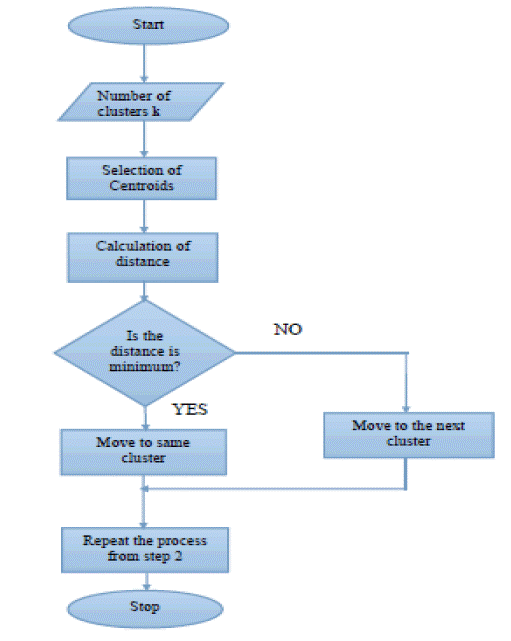
\includegraphics[width=8cm]{images/k-means-flow.png}
    \caption{Biểu đồ khối mô tả thuật toán K-Means}
\end{figure}

Chi tiết các bước thực hiện thuật toán K-Means:
\begin{itemize}[topsep=0ex]
\item Bước 1: Chọn ngẫu nhiên $K$ tâm (centroid) cho $K$ cụm (cluster).
    Mỗi cụm được đại diện bằng các tâm của cụm.

\item Bước 2: Tính khoảng cách giữa các điểm đến tâm $(c_x, c_y)$
    của từng nhóm.
    Dùng khoảng cách Euclidean: 
    $d(a, b) = \sqrt{(a_x - b_x)^2 + (a_y - b_y)^ 2}$

\item Bước 3: Nhóm các điểm vào nhóm có khoảng cách từ tâm
    đến điểm đó nhỏ nhất.

\item Bước 4: Xác định lại tâm mới cho các nhóm, sử dụng công thức:
    $$
    c_x = \frac{a_{1x} + a_{2x} + \cdots + a_{mx}}{m}
    $$
    $$
    c_y = \frac{a_{1y} + a_{2y} + \cdots + a_{my}}{m}
    $$
    với $m$ số phần tử của nhóm.

\item Bước 5: Nếu $(c_x, c_y)$ không đổi thì đó là tâm cần tìm.
    Nếu không thì lặp lại bước 2.
\end{itemize}

Thuật toán này được áp dụng vào chức năng gợi ý phân tuyến
bán hàng cho nhân viên bán hàng của người quản lý tuyến.
Đầu vào của bài toán là $N$ điểm (tương ứng với $N$ cửa hàng bán lẻ)
và $K$ cụm (do người quản lý thiết lập). Cần chia $N$ điểm
này cho $K$ cụm một cách cân bằng và co cụm nhất.
Cụ thể về chức năng này sẽ trình bày ở chương 4 của đồ án.

\section{Các công nghệ sử dụng}
\subsection{Công nghệ front-end}
\subsubsection{ReactJS}
\paragraph{Khái quát về ReactJS}
Ngày nay ReactJS~\cite{reactjs:online} đã trở nên rất phổ biến bởi những tính năng
linh hoạt và đơn giản với hơn 1.300.000 developer và hơn 94.000
trang web đang sử dụng ReactJS
(theo số liệu thống kê trên blog topdev.vn). 
ReactJS là một thư viện JavaScript mã nguồn mở được thiết kế
bởi Facebook để tạo ra những ứng dụng web hấp dẫn, nhanh và
hiệu quả với source code tối thiểu. Mục đích cốt lõi của
ReactJS không chỉ khiến cho trang web phải thật mượt mà còn
phải nhanh, khả năng mở rộng cao và đơn giản. Trên website chính
thức của React tổng quan rằng: ReactJS –
“A JavaScript for library for building user interface”,
tức là React sinh ra để phục vụ tầng View,
tập trung vào xây dựng giao diện. 

Tư tưởng của ReactJS là xây dựng lên các component có
tính tái sử dụng, dễ dàng cho việc chia nhỏ vấn đề, kiểm thử,
giúp chúng ta dễ dàng quản lý, mở rộng hệ thống. Đặc tính của
ReactJS là luôn giữ các component ở trạng thái stateless nhiều
nhất có thể, khiến ta dễ dàng quản lý nó. Bản thân các component
này không có trạng thái, nó nhận đầu vào từ bên ngoài và
chỉ hiển thị ra dựa vào các đầu vào đó, điều này
cũng lý giải tính tái sử dụng (reuse) và tiện lợi
trong kiểm thử (testing) của ReactJS.

\paragraph{Virtual DOM}
Sử dụng ReactJS, ta thường hay nghe tới Virtual DOM~\cite{virtualdom:online},
DOM thì rất quen thuộc với những lập trình viên front-end,
còn Virtual DOM là gì? Có khác gì với DOM không? 

Trước tiên, DOM là viết tắt của Document Object Model là
một chuẩn được định nghĩa bởi W3C dùng để truy xuất và thao
tác trên code HTML bằng các ngôn ngữ lập trình thông dịch
(scripting language) như JavaScript.

Khi DOM thay đổi, trình duyệt phải tính toán lại CSS và dựng lại
trang web, điều này sẽ tốn thời gian, nhất là với những ứng dụng
Single Page Application, việc sửa đổi DOM là liên tục không ngừng
nghỉ. Hay khi xử lý các sự kiện (event) như click, submit, …
DOM sẽ tìm tất cả các node liên quan đến sự kiện và cập nhật nếu
thấy nó cần thiết. Vậy thì có cần thiết khi phải tìm tất
cả các node liên quan không? Hay sẽ hiệu quả hơn khi chỉ tìm
node nào cần cập nhật.

\begin{figure}[H]
\centering
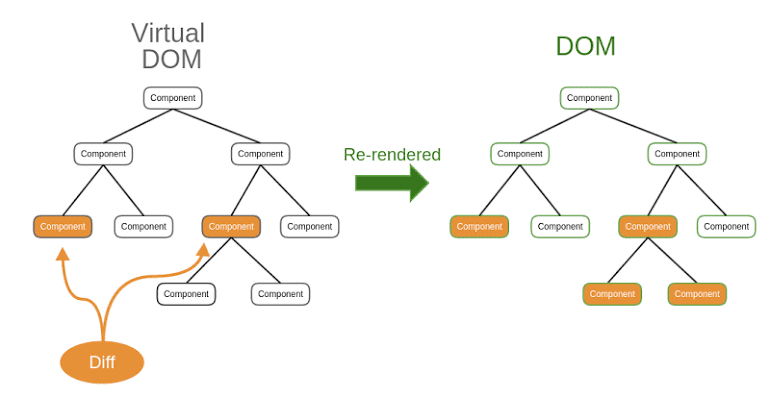
\includegraphics[width=\textwidth]{images/DOM.png}
\caption{Virtual DOM Snapshots \& Diffing}
\label{fig:virtualdom}
\end{figure}

Virtual DOM xuất hiện để giải quyết những vấn đề này.
Virtual DOM gắn với ReactJS, thay vì xử lý DOM Tree thủ công,
chúng định nghĩa các component trông giống DOM
(vì vậy mà cú pháp JSX nhìn rất giống HTML), còn ReactJS sẽ thực
hiện công việc ở tầng thấp hơn. Tổng quát thì Virtual DOM là
một định dạng dữ liệu JavaScript nhẹ dùng để thể hiện nội dung
của DOM tại một thời điểm nhất định nào đó. Nó có tất cả các thuộc
tính giống như DOM nhưng không có khả năng tương tác lên màn hình như
DOM. Sự đặc biệt của Virtual DOM nằm ở cơ chế Snapshots và Diffing.
Khi cần cập nhật phần tử giao diện, React sẽ lấy một snapshot của Virtual
DOM (có thể hiểu là bản ghi trạng thái ngay lúc đó),
sử dụng snapshot này để so sánh với một Virtual DOM trước
khi thực hiện thay đổi.
\paragraph{Single Page Application (SPA)}
Với ReactJS, ta dễ dàng tạo ra một Single Page Application (SPA).
Khác với những ứng dụng web truyền thống, Single Page Application
có một trang gốc và trong trang gốc đó, chúng ta có thể tải
nhiều trang con (tương ứng với các thành phần của trang gốc) mà
không gây bất kì ảnh hưởng gì đến trang gốc. Trong khi các
ứng dụng web truyền thống phải tải lại toàn bộ trang khi
chúng ta tương tác với trang web thì Single Page Application chỉ load
phần trang cần thiết. Các thành phần chung như header, footer, menu,
side bar,… thường xuất hiện ở nhiều trang của ứng dụng sẽ được
Single Page Application load một lần duy nhất ở trang gốc.

\begin{figure}[H]
\centering
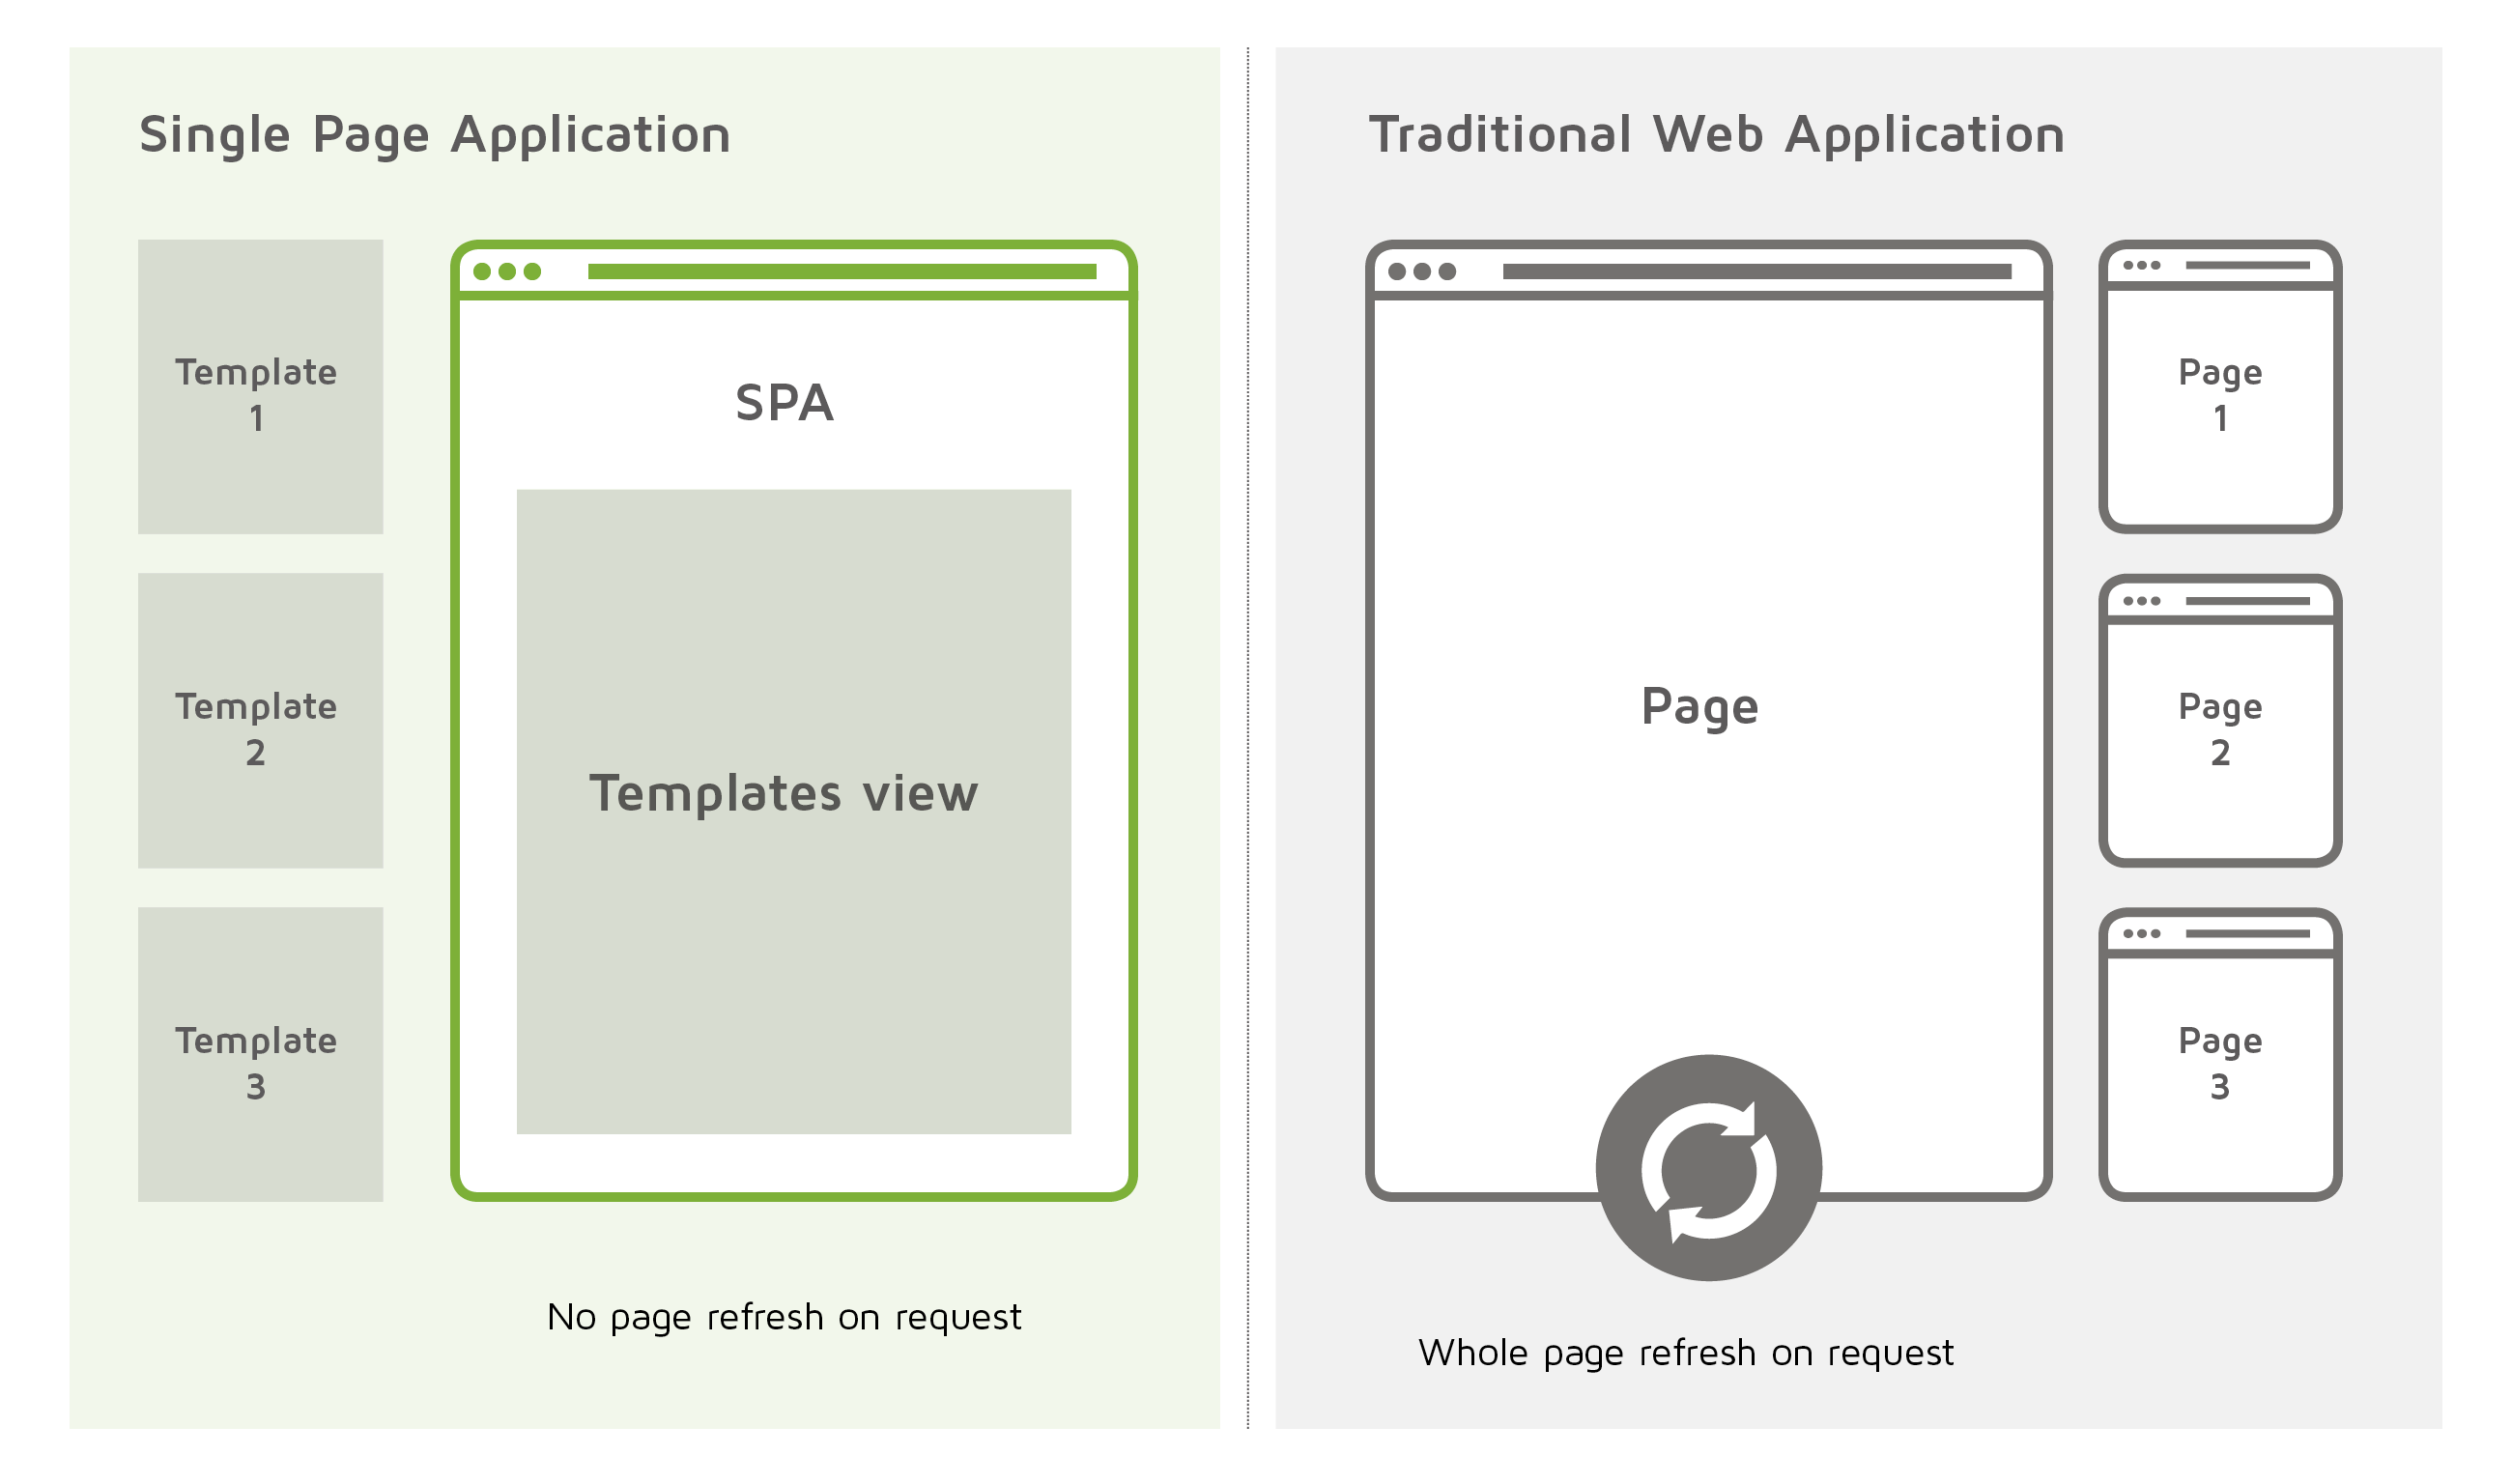
\includegraphics[width=\textwidth]{images/single-page-app.png}
\caption{Single Page Application }
\label{fig:spa}
\end{figure}

Do vậy Single Page Application mang lại nhiều ưu điểm như:
\begin{itemize}[topsep=0ex]
\item Thứ nhất, việc render HTML ở server sẽ cực kì tốn
    tài nguyên nếu trang web có nhiều người dùng, với Single Page
    Application điều này chỉ xảy ra lần đầu tiên khi người dùng
    truy cập trang chủ (hoặc có thể không cần render trên server),
    còn sau đó việc render sẽ do client đảm nhiệm. 

\item Thứ hai, Single Page Application tách biệt front-end và
    back-end, SPA giao tiếp với server chủ yếu qua JSON REST API
    giúp cho dữ liệu gửi và trả giữa client và server giảm
    đến mức tối thiểu. Việc phát triển, kiểm thử cũng có thể
    độc lập giữa front-end và back-end. 

\item Thứ ba, trong suốt quá trình sử dụng, chỉ có dữ liệu là
    được truyền qua lại giữa client và server, còn các tài
    nguyên tĩnh (HTML, CSS, Script, …) chỉ được tải một
    lần duy nhất, vì vậy sẽ giảm thiểu băng thông cho server. 

\item Thứ tư, Single Page Application giúp tăng trải nghiệm người
    dùng, là một ứng dụng web nhưng người dùng tương tác
    giống như một ứng dụng cho Desktop vậy.
\end{itemize}

\paragraph{React Router}
React Router là thư viện định tuyến (routing) chuẩn của React,
nó giúp giao diện của ứng dụng đồng bộ với URL trên trình duyệt.
React Router cho phép định tuyến luồng dữ liệu (data-flow) trong
ứng dụng web một cách rõ ràng. Với React Router, việc xây dựng
Single Page Application trở nên vô cùng dễ dàng.

\begin{figure}[H]
\centering
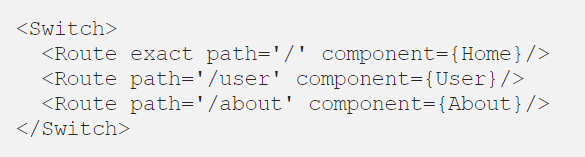
\includegraphics[width=11cm]{images/react-router.png}
\caption{Ví dụ React Router}
\label{fig:reactrouter}
\end{figure}

Hình \ref{fig:reactrouter} trên thể hiện cấu hình 
cơ bản của React Router với
đường dẫn (/path) và Route và giao diện tương ứng.

\subsubsection{Redux}
\paragraph{Khái quát về Redux}
Một ứng dụng web sẽ nhận dữ liệu từ phía máy chủ (back-end),
hay nhận những thao tác của người dùng (input, click, submit, …),
những thứ này chúng ta gọi đó là trạng thái (state) của ứng dụng.
Nếu biết được trạng thái của ứng dụng tại một thời điểm nào đó,
chúng ta sẽ biết vào thời điểm đó ứng dụng đã nhận dữ liệu nào,
những thao tác nào đã được người dùng truyền lên.

Ví dụ: Khi chúng ta click vào nút Back / Forward trên trình duyệt 
thì mỗi trang là một trạng thái của ứng dụng.

Như đã trình bày ở trên, ReactJS xây dựng lên các Single
Page Application, tức chỉ render một trang, và tất cả các
thành phần của ứng dụng sẽ được lưu trữ trong đó. Vì thế,
nếu ứng dụng phức tạp lên theo thời gian, các component sẽ nhiều
lên, và việc quản lý các state của chúng cũng ngày một lớn dần.
Giao diện ứng dụng (UI) cũng trở nên phức tạp vì chúng ta
cần quản lý các công việc active Routes, selected tabs, spinners,
pagination, … Trong ReactJS để truyền dữ liệu giữa các component anh
em, một state phải tồn tại (live) trong một component cha,
một phương thức (method) để update chính state này được cung cung
cấp bởi component cha, từ đây sẽ truyền xuống props của các
component con. Do vậy nếu một state phải được chia sẻ giữa các
component cách khá xa nhau trong một tree component thì state
này sẽ phải được truyền từ một component đến một component khác cho
đến khi nó đến được nơi mà nó được gọi.

\begin{figure}[H]
\centering
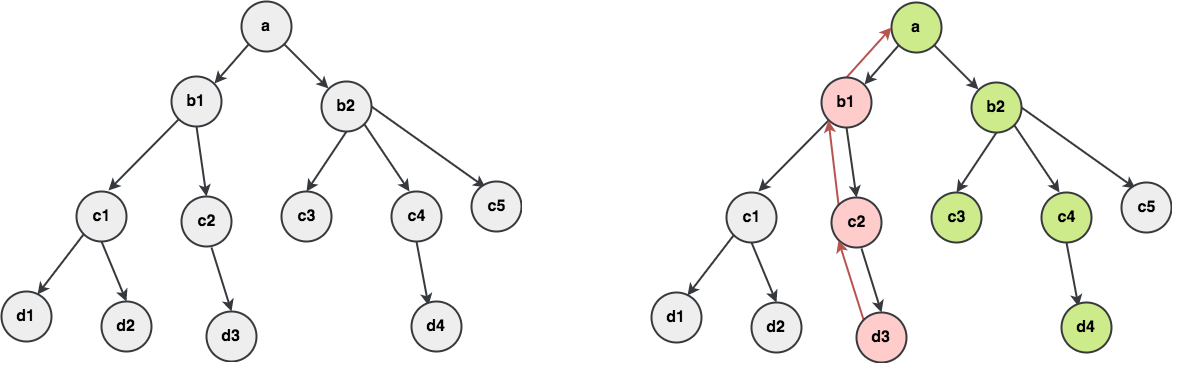
\includegraphics[width=16cm]{images/redux-state-transfer.png}
\caption{Truyền state giữa các component}
\end{figure}

Trong hình vẽ trên, giả sử nếu có một sự kiện ở node d3 kích
hoạt muốn thay đổi state d4 thì luồng dữ liệu sẽ được truyền
từ node d3 trở về node gốc là a, sau đó từ node a lại truyền data
đến các node con. Thứ tự truyền: d3 – c2 – b1 – a – b2 – c4 – d4.
Tương tự nếu muốn thay đổi state ở c3 thì thứ tự truyền là:
d3 – c2 – b1 – a – b2 – c3. Điều này làm cho bộ phận quản lý
state trong ứng dụng trở nên phức tạp và bừa bộn, do vậy ta
cần một công cụ quản lý trạng thái (state management tool)
như Redux. Giải pháp Redux đưa ra như sau:

\begin{figure}[H]
\centering
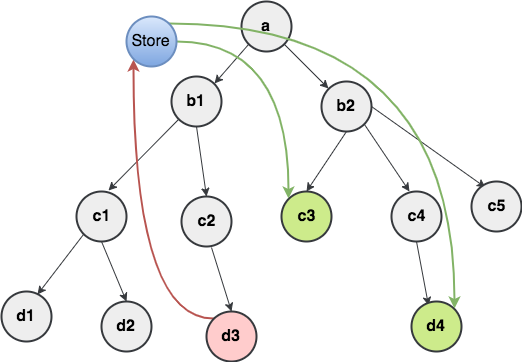
\includegraphics[width=10cm]{images/redux-solution.png}
\caption{Quản lý state trong Redux}
\end{figure}

Quay lại ví dụ ở trên thì ta cần map sự kiện từ node d3
về store của Redux rồi ở node d4, c3 cần connect với store
và cập nhật dữ liệu thay đổi.

\paragraph{Nguyên lý vận hành của Redux}
Cách Redux hoạt động khá đơn giản. Redux có một store lưu trữ
toàn bộ state của ứng dụng. Mỗi component có thể truy cập trực
tiếp đến state được lưu trữ thay vì phải truyền từ component
này qua component khác.

\begin{figure}[H]
\centering
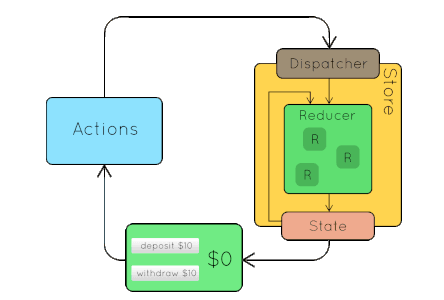
\includegraphics[width=12cm]{images/redux-without-middleware.png}
\caption{Kiến trúc của Redux}
\end{figure}

Redux có 3 thành phần là Action, Store và Reducer.

Action đơn giản là các sự kiện, mô tả những gì xảy ra như 
là cách mà chúng ta gửi dữ liệu từ ứng dụng đến Redux store, 
dữ liệu có thể đến từ sự tương tác của user và ứng dụng, 
API call hoặc khi submit một form, … Tuy nhiên action lại không 
chỉ rõ phần state nào thay đổi, việc này do Reducer đảm nhiệm. 
Reducer nhận vào một state cũ và action được gửi lên 
sau đó trả về một state mới. 

\begin{lstlisting}
(previousState, action) => newState
\end{lstlisting}

Những state này được lưu như những đối tượng (objects) và
chúng định rõ cách state của một ứng dụng thay đổi trong việc
phản hồi một action gửi đến store. Store là nơi lưu lại các
state của ứng dụng và nó là duy nhất
trong bất kì một ứng dụng Redux nào.

\paragraph{Middleware}
Một ứng dụng thực tế đòi hỏi có những thao tác xử lý cần thời
gian để phản hồi (các thao tác bất đồng bộ lấy dữ liệu từ
api hay các thao tác đọc ghi file hay đọc cookie từ trình duyệt, …),
các thao tác như vậy gọi là side effect. Để giải quyết được
các side effect này, trong Redux ta cần thực hiện nó ở middleware.

Trong Redux, Middleware cho phép chúng ta can thiệp vào giữa
thời điểm dispatch một action và thời điểm action đó đến được
reducer. Kiến trúc của Redux đầy đủ khi có middleware như hình dưới đây.

\begin{figure}[H]
\centering
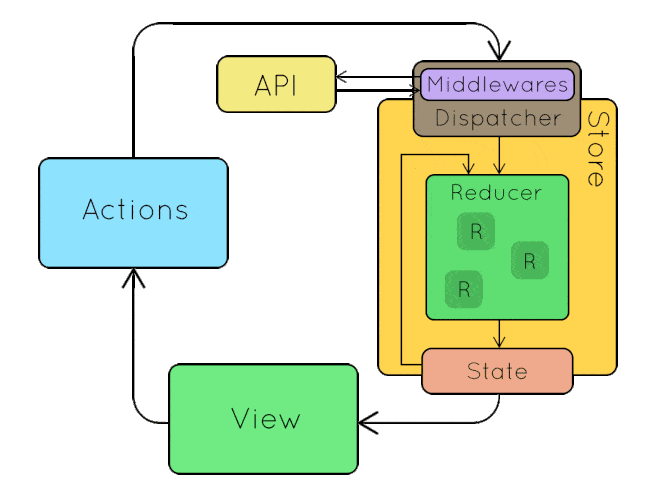
\includegraphics[width=12cm]{images/redux-architecture.png}
\caption{Kiến trúc của Redux với Middleware}
\end{figure}

Ta có thể tự viết một middleware hoặc có thể dùng những thư
viện middleware được xây dựng sẵn. Hiện tại có một vài thư viện
middleware cho Redux, ví dụ như redux-thunk, redux-saga,
redux-observable, … mỗi thư viện có phương pháp giải quyết
vấn đề side-effect riêng.
Trong project này sử dụng redux-saga để xử lý các side-effect.

\paragraph{Redux-saga}
Redux-saga là một thư viện hỗ trợ việc xử lý side-effect trong
ứng dụng React/Redux (ví dụ như xử lý bất đồng bộ khi load dữ liệu,…)
và làm cho các ứng dụng này trở nên đơn giản hơn.
Bằng cách sử dụng Generator Function, redux-saga giúp ta viết
code bất đồng bộ (async code) nhìn giống như là đồng bộ (synchronos).

Generator Function là function có khả năng hoãn lại quá trình
thực thi mà vẫn giữ nguyên được ngữ cảnh của function. Khác với
function bình thường là thực thi và trả về kết quả,
thì Generator function có thể thực thi, tạm dừng trả về
kết quả và thực thi tiếp (bằng cách sử dụng từ khóa \textbf{yield}).
Nếu như function bình thường khi được gọi sẽ thực thi hết tất cả
các câu lệnh trong hàm thì Generator function có khả năng tạm ngưng
trước khi hàm kết thúc và có thể tiếp tục chạy tại một thời điểm khác.
Chính chức năng này giúp ta giải quyết được vấn đề bất đồng bộ,
hàm sẽ dừng và đợi async chạy xong rồi tiếp tục thực thi.

\textit{Nguyên lý hoạt động của Redux-saga:} \\
Redux-saga cung cấp các hàm helper effect, các hàm này sẽ
trả về một effect object chứa các thông tin chỉ dẫn middleware
của Redux có thể thực hiện tiếp các hành động khác. Các hàm
helper effect sẽ được thực thi trong các generator function.
Ví dụ một số helper effect trong Redux-saga:
\begin{itemize}
\item \textit{takeEvery()}:
    thực thi và trả về kết quả của một action được gọi
\item \textit{takeLastest()}: nếu ta thực hiện một loạt các actions,
    nó sẽ chỉ thực thi và trả về kết quả của action cuối cùng.
\item \textit{put()}: dispatch một action.
\item \textit{call()}: gọi một function. Nếu nó trả về một Promise,
    sẽ tạm dừng saga cho đến khi Promise được giải quyết.
\end{itemize}
Ví dụ sử dụng helper effect trong Redux-saga:
\begin{lstlisting}[language=JavaScript,caption={Sử dụng Redux-Saga},captionpos=b]
// execute fetchPersonListSaga
// when action FETCH_PERSON_LIST is dispatched
yield takeEvery(FETCH_PERSON_LIST, fetchPersonListSaga);

// dispatch action pushSuccessNotification 
yield put(pushSuccessNotification(sequence, "Saved"));
\end{lstlisting}

% \subsubsection{Material-UI}
% \paragraph{Material Design}
% Material UI là một thư viện các React Component và được 
% tích hợp thêm cả Google’s Material Design. Trước tiên, 
% chúng ta sẽ tìm hiểu về nguyên lý Material Design. 

% Material Design là phong cách thiết kế áp dụng chủ yếu trong thiết
% kế ứng dụng Web, ứng dụng Mobile và đã trở thành một xu hướng
% phổ biến hiện nay. Đối với những Designer thiết kế UX/UI
% (giao diện / trải nghiệm người dùng), hay các lập trình viên
% front-end thì thuật ngữ Material Design không còn xa lạ.
% Có rất nhiều ứng dụng nổi tiếng thiết kế theo phong
% cách Material Design như các ứng dụng của Google
% (Google+, Gmail, Google Maps, …), Evernote, ePay, …

% \begin{figure}[H]
% \centering
% 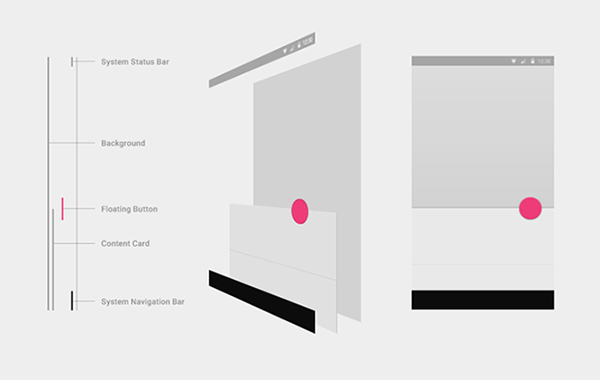
\includegraphics[width=14cm]{images/material-design.png}
% \caption{Thiết kế Material Design}
% \end{figure}

% Material Design là hình thức phát triển cao hơn của
% Flat Design (thiết kế phẳng), tuy nhiên thay vì cảm
% giác “phẳng lì” trên toàn bộ giao diện, Material Design là
% những lớp xếp chồng lên nhau, tạo chiều sâu, điểm nhấn hơn
% những thiết kế phẳng thông thường. Material Design chủ yếu tập
% trung vào những đường nét đơn giản, sử dụng những gam màu đậm,
% nổi bật, đồng thời cũng thường sử dụng những yếu tố đồ họa
% có cảm giác 3D, có hiệu ứng “nổi lên” (float) trên giao diện.
% Ngoài ra, thiết kế này còn bao gồm những chuyển động tự nhiên,
% tất cả những điều này đều nhằm mục đích mang lại cho người
% dùng trải nghiệm mới mẻ, thú vị và gần gũi hơn.

% Material Design có 3 yếu tố căn bản:
% \begin{itemize}[topsep=0ex]
% \item Thứ nhất là không gian: 
%     Không gian dưới lớp kính màn hình thiết bị được mô phỏng
%     như một không gian 3 chiều Oxyz với chiều sâu là trục Oz.
%     Để tạo chiều sâu cho thiết kế, designer cần điều chỉnh ánh
%     sáng một cách phù hợp.

% \begin{figure}[H]
% \centering
% 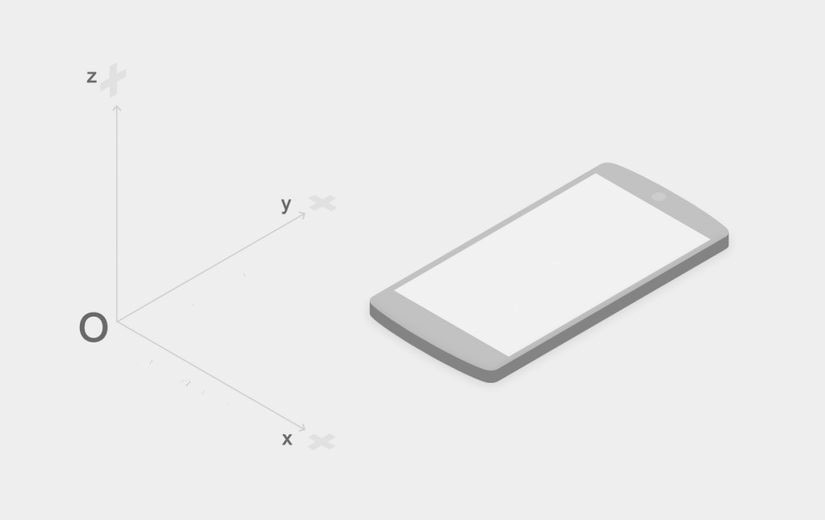
\includegraphics[width=12cm]{images/material-design-space.jpg}
% \caption{Material Design – Không gian}
% \end{figure}

% \item Thứ hai là ánh sáng:
%     Ánh sáng là yếu tố môi trường được sử dụng nhằm thể
%     hiện tính 3 chiều của không gian. Hệ quả của ánh sáng là hiệu ứng
%     đổ bóng (Drop Shadow), sẽ phân định vị trí các lớp Material trong
%     không gian theo trục Oz. Có hai loại nguồn sáng được kết hợp
%     là nguồn sáng chiếu trực tiếp và ánh sáng môi trường. Nguồn sáng
%     trực tiếp rất quan trọng, nó giống như nguồn sáng đèn pin,
%     nó mang lại hiệu ứng đổ bóng mạnh và sắc nét. Ánh sáng môi trường
%     thì nhẹ nhàng và không rõ nguồn, tạo viền bóng nhẹ xung quanh.
%     Thông thường, Material Design kết hợp cả hai nguồn sáng, mang
%     đến hiệu ứng bóng tổng hợp, mô phỏng không gian thực tế.

% \begin{figure}[H]
% \centering
% 
\includegraphics[width=14cm]{images/material-design-light.jpg}
% \caption{Material Design – Ánh sáng}
% \end{figure}

% \item Thứ ba là material (chất liệu): Là những mặt phẳng có độ dày
%     đồng nhất 1dp (1 in $\approx$ 160 dp) và nằm song song với mặt phẳng Oxy.
%     Các mặt phẳng Material sắp xếp chồng lên nhau theo trục Oz.
%     Thông qua việc thay đổi kích thước của bóng, ta sẽ dễ dàng
%     mô tả vị trí tương đối của mỗi lớp so với lớp khác.

% \begin{figure}[H]
% \centering
% 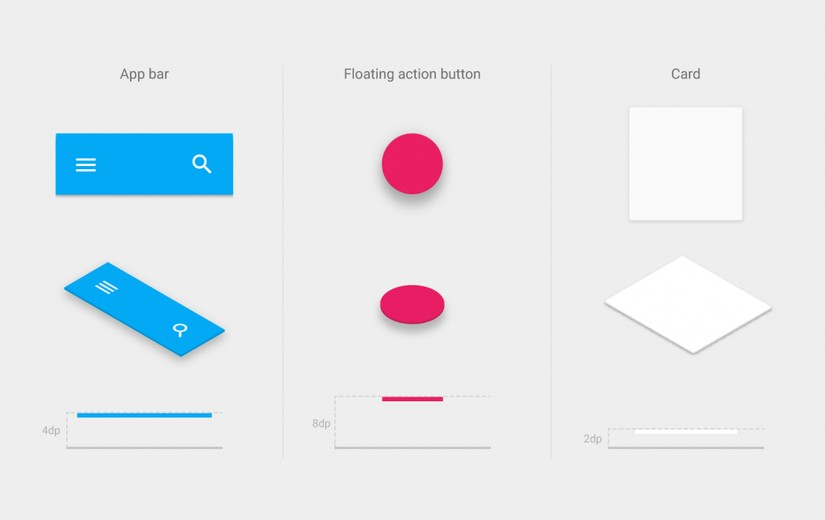
\includegraphics[width=14cm]{images/material-design-material.png}
% \caption{Material Design – Chất liệu}
% \end{figure}

% \end{itemize}

% Để có một thiết kế ấn tượng với Material Design cần
% chú ý một vài hiệu ứng và chi tiết:
% \begin{itemize}[topsep=0ex]
% \item Hiệu ứng tự nhiên: ví dụ khi bạn nhấn chọn một thành phần,
%     hiệu ứng sóng trên màn hình sẽ tỏa ra tự vị trí ngón tay
%     bạn chứ không phải từ một hướng cố định.

% \item Hiệu ứng bề mặt: khi chuyển trang, các thành phần phải chuyển
%     động một cách tự nhiên và liên tục chứ không biến mất

% \item Có thứ tự: những thành phần ở sau sẽ xuất hiện trước,
%     thành phần lớn hơn sẽ xuất hiện trước, thành phần quan trọng
%     hơn sẽ xuất hiện trước.

% \item Thống nhất: chuyển động của những Material phải thống nhất
%     từ cùng một hướng, tạo sự đồng đều cho tổng thiết kế.
% \end{itemize}

% \paragraph{Material-UI}
% Như đã trình bày ở trên, Material UI là một thư viện các
% React component tích hợp thêm Google’s Material Design.
% Material UI cung cấp khá đầy đủ các component để có thể tạo
% ra một trang web một cách nhanh chóng hơn mà không phải ngồi
% chỉnh CSS từng chút một.

% Ví dụ để tạo ra các nút bấm như hình dưới,
% ta chỉ việc sử dụng Button component mà Material UI cung cấp.
% \begin{figure}[H]
% \centering
% 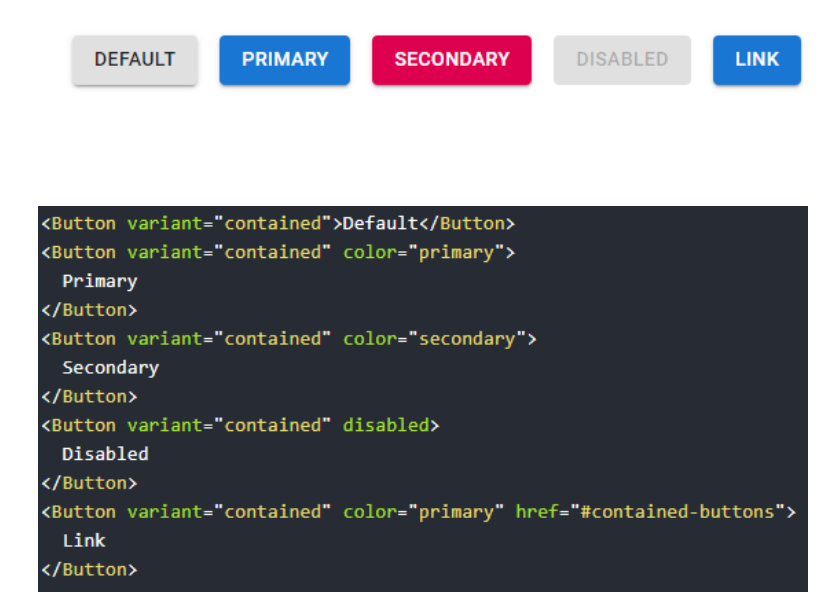
\includegraphics[width=14cm]{images/material-ui-button.png}
% \caption{Material UI – Button}
% \end{figure}

% Việc thêm màu sắc là vô cùng đơn giản với những thuộc
% tính được định nghĩa sẵn, màu sắc là chuẩn theo thiết
% kế Material Design. 
% Với Material UI, chúng ta còn dễ dàng chia bố cục và
% responsive trang web. Grid component sẽ chia màn hình theo
% bố cục 12 cột, 5 loại màn hình theo
% kích cỡ (xs, sm, md, lg, xl).

% Cùng một nội dung nhưng khi được hiển thị trên các màn
% hình khác nhau sẽ hiển thị theo cách khác nhau, đảm bảo sự thuận
% tiện nhất cho người dùng.  Thuật ngữ “Responsive Design” ám
% chỉ cách thiết kế trang web hiển thị tương thích với mọi kích thước
% thiết bị, tức là bố cục trang web sẽ tự đáp ứng theo hành vi
% người dùng và môi trường hiển thị. Môi trường này chính là kích thước
% của trình duyệt, kích thước hoặc hướng xoay thiết bị. Thiết
% kế Responsive không chỉ giúp cho người dùng có một trải nghiệm thú
% vị hơn khi truy cập website, mà còn giúp chủ sở hữu dễ dàng
% quản lý các trang web của mình hơn.

% Ngoài ra Material UI cũng có sẵn kho Icon khổng lồ trên đầy
% đủ các lĩnh vực giúp chúng ta dễ dàng chọn ra icon đẹp và
% phù hợp nhất với mỗi nội dung trên trang web.


\subsection{Công nghệ lưu trữ - Redis}
Redis~\cite{redis:online} là viết tắt của Remote Dictionary Server
(máy chủ từ điển từ xa), lưu trữ dữ liệu dưới dạng
KEY-VALUE trong bộ nhớ. Là phần mềm mã nguồn mở có tốc độ
truy cập nhanh để dùng làm cơ sở dữ liệu đơn giản, bộ nhớ đệm (cache),
trình chuyển tiếp (broker) tin nhắn hoặc
được sử dụng làm danh sách tác vụ chờ xử lý (queue). 

Redis hiện cung cấp thời gian phản hồi ở tốc độ chưa đến
một mili giây, giúp thực hiện hàng triệu yêu cầu mỗi giây cho
các ứng dụng thời gian thực trong lĩnh vực Trò chơi, Quảng cáo, Dịch
vụ tài chính, Chăm sóc sức khoe, IoT, … Cụ thể, Redis thường được chọn
sử dụng cho các hoạt động lưu trữ bộ nhớ đệm, quản lý phiên, trò chơi,
bảng xếp hạng, phân tích thời gian thực, dữ liệu không gian
địa lý, ứng dụng đặt xe, trò chuyện / nhắn tin, phát trực tiếp
nội dung đa phương tiện, …

Redis là một cơ sở dữ liệu NoSQL. NoSQL là một dạng cơ sở dữ liệu
phi quan hệ, sử dụng nhiều loại mô hình dữ liệu đa dạng để
truy cập và quản lý dữ liệu trong bộ nhớ và tìm kiếm, NoSQL được
tối ưu hóa dành riêng cho các ứng dụng yêu cầu mô hình dữ liệu
linh hoạt có lượng dữ liệu lớn và độ trễ thấp, đạt được bằng cách
giảm bớt một số hạn chế về tính nhất quán của dữ liệu.

\begin{figure}[H]
    \centering
    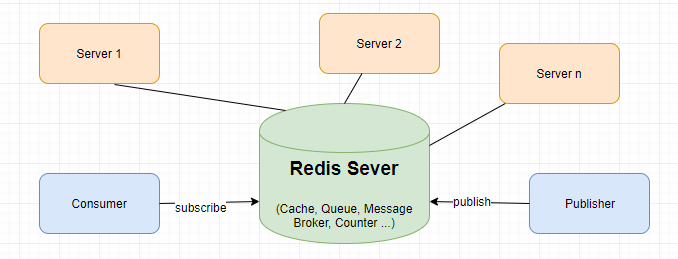
\includegraphics[width=14cm]{images/redis.png}
    \caption{Redis server}
\end{figure}

\textit{Cách thức hoạt động của Redis:}

Toàn bộ dữ liệu của Redis nằm trong bộ nhớ (RAM), khác với những loại 
cơ sở dữ liệu thông thường khác lưu dữ liệu trên ổ đĩa hoặc ổ SSD. 
Phần lớn các tác vụ trên cơ sở dữ liệu truyền thống đều yêu cầu 
truy cập qua lại tới ổ đĩa, do vậy sẽ tốn thời gian tìm kiếm, 
dữ liệu của Redis nằm trên RAM nên sẽ không mất thời gian này. 
Do đó Redis có thể hỗ trợ thêm khá nhiều tác vụ và có thời gian 
phản hồi nhanh hơn. Hiệu suất của Redis rất tốt với các tác 
vụ đọc ghi thông thường mất chưa đầy một mili giây và hỗ trợ 
hàng triệu tác vụ mỗi giây. 

Khác với các cơ sở dữ liệu quan hệ như MySQL hay PostgreSQL,
Redis không có bảng. Redis lưu dữ liệu dưới dạng KEY-VALUE và hỗ
trợ nhiều cấu trúc dữ liệu cơ bản như hash, list, set,
sorted set, string, … Bên cạnh đó Redis có 2 background threads chuyên
làm nhiệm vụ định kì ghi dữ liệu trên đĩa cứng, cơ chế backup
này giúp cho Redis có độ bảo mật và sửa lỗi cao.

\textit{Một số ứng dụng phổ biến của Redis:}
\begin{itemize}[topsep=0ex]
\item Lưu trữ bộ nhớ đệm (caching): Sử dụng bộ nhớ đệm để giảm độ trễ
    khi truy cập dữ liệu, tăng năng suất và giảm tải cho cơ sở dữ
    liệu và ứng dụng của bạn. Redis có thể phục vụ những dữ liệu thường
    xuyên được yêu cầu với thời gian phản hồi chưa đến một mili giây
    và cho phép dễ dàng thay đổi quy mô nhằm đáp ứng mức tải cao hơn
    mà không cần tốn kém chi phí vào back-end.

\item Bảng xếp hạng game: Redis là giải pháp hay được các nhà phát
    triển game dùng để xây dựng bảng xếp hạng theo thời gian thực
    (real-time leaderboard). Sử dụng cấu trúc dữ liệu Sorted Set của
    Redis, cấu trúc dữ liệu này đảm bảo tính duy nhất của các thành
    phần trong khi vẫn duy trì danh sách được sắp xếp theo điểm số
    của người dùng. Danh sách cập nhật mỗi khi điểm số người dùng thay đổi.

\begin{figure}[H]
    \centering
    
\includegraphics[width=10cm]{images/real-time-leader-board.png}
    \caption{Ứng dụng Redis trong bảng xếp hạng game}
\end{figure}

\item Lưu trữ phiên (session): Các nhà phát triển ứng dụng thường sử
    dụng Redis để lưu trữ, quản lý phiên cho các ứng dụng quy mô
    Internet. Quản lý dữ liệu phiên chẳng hạn như hồ sơ người dùng,
    thông tin xác thực đăng nhập (token), trạng thái phiên, …

\item Trò chuyện, nhắn tin, hàng chờ xử lý tác vụ: Redis hỗ trợ Pub/Sub
    (là cấu trúc gửi – nhận tin nhắn mà người gửi và người nhận không
    biết nhau) với nhiều cấu trúc dữ liệu như list, sorted set, hash.
    Điều này cho phép Redis hỗ trợ những chat rooms hiệu năng cao,
    luồng tin nhắn theo thời gian thực.
\end{itemize}

\textit{So sánh Redis và một loại cơ sở dữ liệu quan hệ thông thường (MySQL)}
\begin{table}[H]
\centering
\begin{tabular}{| m{3cm} | m{6cm} | m{6cm} |}
\hline
& \textbf{Redis} & \textbf{MySQL} \\ 

\hline
\multirow{5}{3cm}{Cấu trúc cơ sở dữ liệu} &
Lưu trữ dạng KEY-VALUE & Lưu trữ dạng bảng \\  
\cline{2-3}
& Lưu dữ liệu trong RAM, là máy chủ cấu trúc dữ
liệu vì các key có thể chứa string, hash, list,
set và sorted set
& MySQL cung cấp một máy chủ cơ sở dữ liệu quan hệ SQL
rất nhanh, đa luồng, đa người dùng, mạnh mẽ \\  

\hline
\multirow{9}{3cm}{Ưu điểm}
& $\bullet$ Dễ cài đặt, sử dụng, deploy, maintain, … & 
$\bullet$ Cơ sở dữ liệu quan hệ mã nguồn mở được sử dụng rộng rãi \\
& $\bullet$ Lưu trữ dữ liệu trong bộ nhớ nên cho hiệu
    năng cao và tốc độ nhanh &
$\bullet$ Dễ sử dụng, khả năng tương thích cao, hỗ trợ đa nền tảng,
cộng đồng phát triển mạnh mẽ \\
& $\bullet$ Mã nguồn mở, ổn định, chi phí hiệu quả &
$\bullet$ Hỗ trợ index và full-text searching \\
& $\bullet$ Khả năng mở rộng cao, hỗ trợ sao lưu vào đĩa cứng & \\
& $\bullet$ Cấu trúc dữ liệu đa dạng & \\
\hline
\multirow{5}{3cm}{Trường hợp nên sử dụng} & 
$\bullet$ Có dữ liệu dạng KEY-VALUE & $\bullet$ Cần cơ sở dữ liệu quan hệ \\
& $\bullet$ Cần lưu cache & $\bullet$ Khi có các hoạt động phân tán \\
& $\bullet$ Cần hiệu năng cao &
$\bullet$ Cần bảo mật cao và hoạt động đơn giản \\
& $\bullet$ Kích thước dữ liệu ổn định &
$\bullet$ Không sử dụng khi dữ liệu lớn dần và 
không thể cache hết lên bộ nhớ \\
\hline
\multirow{3}{3cm}{Nhược điểm} & 
$\bullet$ Redis sử dụng RAM nên khi lượng file cache lớn sẽ
dẫn đến thiếu RAM cho server &
$\bullet$ Nhiều vấn đề về lưu trữ procedure và trigger \\
& $\bullet$ Không thể truy vấn trực tiếp các object & \\
\hline
\end{tabular}
\caption{So sánh Redis và MySQL}
\end{table}

\subsection{Công nghệ lưu trữ - PostgreSQL}

\subsubsection{Tổng quan về PostgreSQL}
PostgreSQL, còn được gọi là Postgres, là một hệ thống quản lý cơ sở 
dữ liệu quan hệ miễn phí mã nguồn mở chú trọng vào tính mở rộng và 
tính tương thích với chuẩn SQL. Ban đầu có tên là POSTGRES, có nguồn
gốc từ cơ sở dữ liệu Ingress được phát triển tại

Đại học California, Berkeley. Vào năm 1996, dự án được đổi tên thành
PostgreSQL. PostgreSQL được viết bằng ngôn ngữ C và có thể chạy trên nhiều
hệ điều hành như Linux, macOS, Windows, \ldots Đồng thời hỗ trợ các tính
năng tương tự như nhiều các cơ sở dữ liệu quan hệ khác.
Phiên bản PostgreSQL sử dụng trong đồ án này là 11.8.

\subsubsection{Tổng quan về Index}
Index trong cơ sở dữ liệu là một cấu trúc dữ liệu giúp cải thiện
tốc độ truy vấn dữ liệu trên các bảng với đánh đổi là sử dụng thêm
không gian lưu trữ nhằm duy trì cấu trúc dữ liệu index cũng như
làm tăng thời gian ghi dữ liệu. Index được sử dụng để nhanh chóng
định vị dữ liệu mà không phải tìm duyệt qua toàn bộ các hàng trong
bảng của cơ sở dữ liệu mỗi khi bảng đó được truy cập. Index có thể
được tạo sử dụng một hay nhiều cột trong cùng một bảng, cung cấp
cơ chế tăng tốc quá trình tra cứu ngẫu nhiên và truy cập có thứ
tự các bản ghi trong cơ sở dữ liệu. 

Index được chia làm hai loại kiến trúc:
Clustered Index và Non-clustered Index.

Với clustered index, các hàng trong cơ sở dữ liệu được lưu trữ
trên đĩa theo cùng thứ tự với index. Do đó mỗi bảng chỉ tồn tại
duy nhất một clustered index. Với non-clustered index thì cấu trúc dữ
liệu index là cấu trúc dữ liệu nằm ngoài bảng, các hàng trong bảng
không được đảm bảo thứ tự giống như thứ tự của index. Một bảng có
thể có rất nhiều non-clustered index. Thông thường với truy cập trên
clustered index sẽ nhanh hơn trên non-clustered index vì dữ liệu
sẽ không bị phân mảnh ở nhiều vị trí trong ổ cứng.

\subsubsection{Index trong PostgreSQL}
Trong PostgreSQL, clustered index không được hỗ trợ. Tuy nhiên
PostgreSQL lại hỗ trợ nhiều kiểu index như B-Tree, Hash, GiST,
SP-GiST, GIN và BRIN. Mỗi một kiểu index sử dụng một thuật toán
riêng biệt để tối ưu cho nhiều loại câu truy vấn khác nhau.
Mặc định khi sử dụng lệnh CREATE INDEX thì index B-Tree sẽ được tạo,
index này cũng phù hợp với hầu hết các
trường hợp truy vấn~\cite{postgresdocs}.

Index kiểu B-Tree có thể được xử dụng cho các câu truy vấn
liên quan đến tìm kiếm bằng, tìm kiếm khoảng hoặc trong trường
hợp dữ liệu được sắp xếp theo một trường nào đó. Trình lập kế hoạch
cho các truy vấn của PostgreSQL sẽ xem xét sử dụng index B-Tree
bất kì khi nào trường mà có index nằm trong một trong
các phép toán so sánh như $<$ $<=$ $=$ $>=$ $>$.

Các toán tử tương đương hoặc tổ hợp của chúng, như là phép toán
BETWEEN và IN, cũng có thể sử dụng được index B-Tree.
Ngoài ra các phép toán liên quan đến NULL như IS NULL hay
IS NOT NULL cũng có thể được tăng tốc bằng index B-Tree.

Trình tối ưu cũng có thể sử dụng index B-Tree cho các câu
truy vấn sử dụng toán tử pattern matching như LIKE và ~
nếu mà pattern được sử dụng bắt đầu là một xâu hằng số
như ‘foo\%’ nhưng không phải là ‘\%bar’. 

B-Tree có thể cũng được sử dụng để lấy dữ liệu được sắp
xếp theo thứ tự của cột được index.

Index kiểu Hash chỉ có thể được sử dụng trong các câu truy
vấn sử dụng toán tử so sánh bằng. Để tạo index Hash trong PostgreSQL,
ta sử dụng:
\begin{lstlisting}[caption={Tạo index sử dụng Hash}, captionpos=b]
CREATE INDEX name ON table USING HASH (column);
\end{lstlisting}

\subsubsection{Full Text Search trên PostgreSQL}
\paragraph{Cơ bản về Full Text Search}
Các toán tử tìm kiếm text trên các CSDL quan hệ đã tồn
tại từ rất lâu như LIKE hay ILIKE. Nhưng những toán tử đó thiếu
đi những tính chất mà cần có trong các hệ thống thông tin hiện đại như:
\begin{itemize}[topsep=0ex]
\item Hỗ trợ ngôn ngữ, thậm chí với cả tiếng Anh. Các toán tử
    trên không phù hợp cho việc xử lý những từ gần giống nghĩa hoặc
    được suy diễn, như satisfy và satisfies trong tiếng Anh. Có thể
    dùng toán tử logic OR để tìm kiếm cả 2 nhưng phải liệt kê rất
    nhiều trường hợp và một số từ có thể có rất nhiều từ
    được suy diễn hoặc gần nghĩa.

\item Không hỗ trợ xếp hạng (ranking) trên tập kết quả,
    dẫn đến tìm kiếm không hiệu quả khi mà có thể có tới rất
    nhiều document được tìm thấy trong một câu truy vấn.

\item Các phép toán đó thường chậm vì không hỗ trợ đánh chỉ
    số, mỗi một câu truy vấn phải duyệt qua toàn bộ các document.
\end{itemize}

PostgreSQL hỗ trợ tiền xử lý các document và đánh chỉ
số để tăng tốc các câu truy vấn. Tiền xử lý document bao gồm việc:
\begin{itemize}[topsep=0ex]
\item Phân tích document thành các token.
\item Chuyển các token thành các lexeme.
\item Lưu trữ các dữ liệu sau khi tiền xử lý
    document để tối ưu cho truy vấn.
\end{itemize}

Một document trong PostgeSQL thông thường là một cột chứa
xâu của bảng CSDL, hoặc có thể là một 
tổ hợp (thông qua phép ghép nối xâu) của những trường
đó trong một bảng hay trong nhiều bảng hoặc
có thể được truyền từ ngoài vào. 

Một token là một xâu biểu diễn một từ được phân tích ra từ document.

Một lexeme cũng là một xâu, tương tự như token, nhưng đã
được chuẩn hóa (normalize) sao cho những dạng khác nhau của
một từ trở thành giống nhau. Việc chuẩn hóa luôn luôn
thực hiện chuyển tất cả các kí tự thành lower-case, và thông
thường có cắt bỏ một vài các hậu tố như e hoặc es trong tiếng
Anh. Đồng thời ở bước chuyển từ token thành càng lexeme cũng
thông thường loại bỏ những stop word, là những từ rất phổ biến
trở thành vô nghĩa khi tìm kiếm, PostgreSQL sử dụng Dictionary
để thực thi bước này.

Dictionary trong PostgreSQL cho phép hiệu chỉnh quá trình
chuẩn hóa thành lexeme, bao gồm:
\begin{itemize}[topsep=0ex]
\item Định nghĩa các stop word được loại bỏ.
\item Ánh xạ các từ đồng nghĩa thành một từ.
\item Ánh xạ cụm từ thành một từ.
\item Ánh xạ các biến thể của một từ thành dạng chuẩn.
\end{itemize}

PostgreSQL sử dụng kiểu dữ liệu tsvector để lưu trữ dữ
liệu sau khi tiền xử lý document, đồng thời sử dụng kiểu
tsquery để biểu diễn các câu truy vấn.

Để chuyển từ một xâu sang kiểu tsvector ta sử dụng hàm
to\_tsvector. Còn để chuyển một xâu bất kì sang một tsquery,
ta sử dụng plainto\_tsquery. 

Để thực hiện Full Text Search một tsvector với một tsquery,
ta sử dụng toán tử @@.

\paragraph{Full Text Search cho tiếng Việt}
Để thực hiện Full Text Search với tiếng Việt,
trong đồ án này sử dụng một hàm được định nghĩa bằng SQL như sau: 
\begin{figure}[H]
\centering
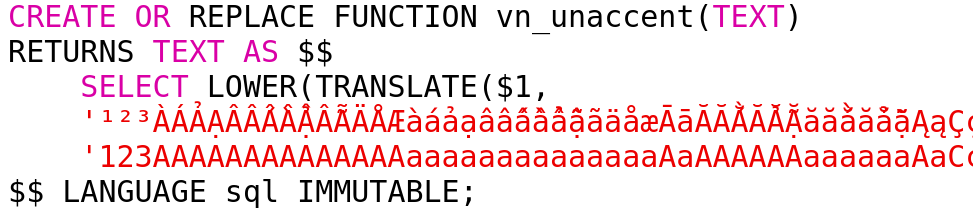
\includegraphics[width=10cm]{images/unaccent.png}
\end{figure}
Khi đó, thay vì sử dụng trực tiếp to\_tsvector và plainto\_tsquery,
ta sử dụng \\
to\_tsvector(vn\_unaccent(text)) và plainto\_tsquery(vn\_unaccent(text)).

\paragraph{Đánh chỉ số cho Full Text Search}
Để sử dụng Index cho Full Text Search, trước tiên ta cần tạo
một cột trong CSDL lưu trữ kiểu dữ liệu tsvector.
Có hai loại Index hay được sử dụng cho Full Text Search là GIN và GiST. 

\noindent Để Index sử dụng GIN, cú pháp như sau:
\begin{lstlisting}[caption={Tạo index sử dụng GIN},captionpos=b]
CREATE INDEX idx_textsearch ON sometable USING GIN (tsvector_column);
\end{lstlisting}

\noindent Còn nếu sử dụng GiST:
\begin{lstlisting}[caption={Tạo index sử dụng GiST},captionpos=b]
CREATE INDEX idx_textsearch ON sometable USING GIST (tsvector_column);
\end{lstlisting}

Khi đó toán tử @@ có thể sử dụng Index để
tăng tốc câu truy vấn. Trong PostgreSQL, Index Full Text Search
thông thường sử dụng GIN hơn sử dụng GiST. 

Thông thường sẽ sử dụng trigger để cập nhật các trường
tsvector trong CSDL khi chèn hoặc chỉnh sửa.

\paragraph{GIN}
\begin{figure}[H]
\centering
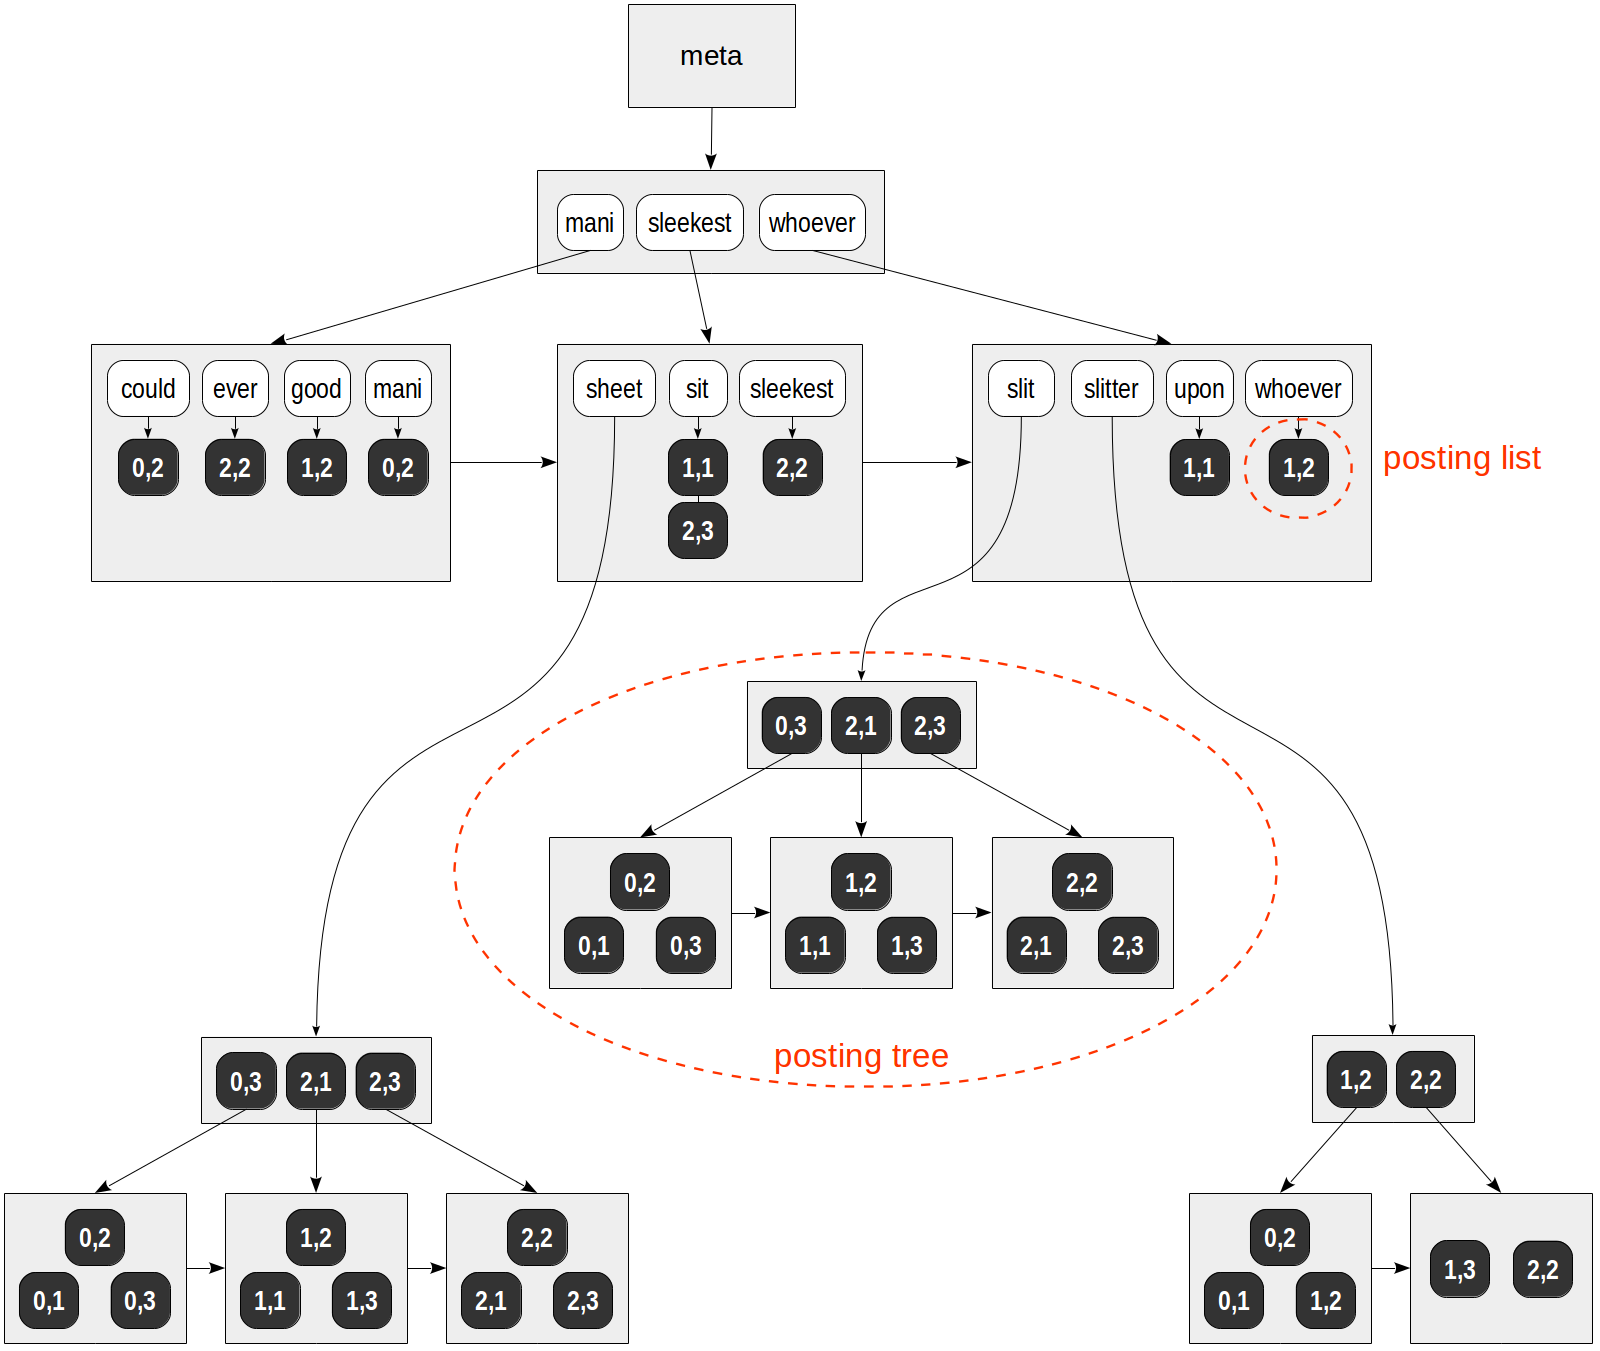
\includegraphics[width=13cm]{images/GIN.png}
\caption{Cấu trúc của GIN}
\end{figure}

GIN là viết tắt của Generalized Inverted Index. GIN được thiết
kế cho việc đánh chỉ số những giá trị tổng hợp (composite value),
và cho phép tìm kiếm cho các phần tử xuất hiện
trong các compostive value. 

Nếu quy ước một composite value là một item, còn phần tử trong
composite value là một key thì GIN 
luôn luôn lưu trữ và tìm kiếm trên key chứ không phải trên item.
Một GIN index lưu trữ tập các cặp (key, posting list) trong đó
posting list là tập các ID của các hàng trong bảng của CSDL.
Một ID có thể được nằm trong nhiều các posting list vì một
item có thể có nhiều các key. Mỗi một key được lưu trữ một
lần duy nhất, do đó nên GIN rất phù hợp trong trường hợp một
key xuất hiện nhiều lần. posting list được lưu với thứ tự
từ nhỏ đến lớn các ID của các hàng. Nếu posting list quá lớn
sẽ được chuyển thành posting tree, cấu trúc tương tự như B-Tree. 

\subsection{Công nghệ back-end}
\subsubsection{Giới thiệu về ngôn ngữ Go}
Go là ngôn ngữ biên dịch kiểu tĩnh được tạo ra tại Google.
Cú pháp của Go tương tự như của ngôn ngữ C, đồng thời cũng
bị ảnh hưởng lớn bởi ngôn ngữ này. Ngôn ngữ Go cũng thông
thường được gọi với tên là Golang.
Sau đây là một số đặc điểm của ngôn ngữ Go:
\begin{itemize}[topsep=0ex]
\item Cú pháp và môi trường lập trình của Go có
    tính tương đồng với các ngôn ngữ lập trình
    kiểu động (dynamic language) như:
    \begin{itemize}[topsep=0ex]
    \item Rút gọi khai báo biến, không cần phải khai báo kiểu
        thông qua cơ chế type inference.
    \item Biên dịch nhanh.
    \item Quản lý các gói thư viện từ xa và các
        package có document truy cập online.
    \end{itemize}

\item Sử dụng cách tiếp cận đặc biệt với một số vấn đề:
    \begin{itemize}[topsep=0ex]
    \item Xây dựng sẵn trong ngôn ngữ một số cơ chế cho lập trình
        đồng bộ như: tiến trình nhẹ (light-weight process,
        hay còn gọi là goroutine), channel và câu lệnh select.
    \item Toolchain mặc định khi biên dịch sinh ra file thực
        thi sẽ không chứa phụ thuộc ngoài.
    \end{itemize}

\item Ngôn ngữ được thiết kế đủ đơn giản để lập trình
    viên có thể dễ dàng hiểu và ghi nhớ.
\end{itemize}

\subsubsection{Goroutine, Chanel và khối lệnh Select}
Ngôn ngữ Go được xây dựng sẵn trong ngôn ngữ những cơ chế hỗ trợ việc
lập trình đồng bộ. Đồng bộ ở đây không chỉ là song song ở mức CPU mà
đồng thời cả việc sử dụng Asynchronous I/O cho phép các câu lệnh như
truy cập database hay đọc gói tin từ mạng chạy trong khi tiến
trình vẫn được sử dụng cho công việc khác. Kỹ thuật này phổ biến
trong các server mà sử dụng event-based.

Trung tập của xây dựng chương trình đồng bộ trong Go là tiến trình
nhẹ (light-weight process) gọi là Goroutine. Một lời gọi hàm mà
được đặt sau từ khóa go sẽ bắt đầu hàm đó trong một Goroutine mới.
Trong đặc tả ngôn ngữ (Language Specfication) không chỉ định Goroutine
được cài đặt như nào nhưng với cài đặt hiện tại thì các Goroutine
sẽ được phân bố vào một tập nhỏ các luồng ở mức hệ điều hành,
tương tự như cơ chế phân phát tiến trình trong ngôn ngữ Erlang.
Khi chương trình Go mới bắt đầu sẽ chứa duy nhất
một goroutine gọi là main goroutine.

Chương trình viết bằng Go sẽ thường sử dụng Channel, một cơ chế để
gửi các thông điệp (Message) giữa các goroutine. Channel trong Go có thể
có chứa Buffer hoặc không. Nếu không chứa Buffer thì Channel mỗi một
thời điểm chỉ chứa tối đa một Message, các lời gọi gửi message vào
channel tiếp theo đó sẽ bị block. Nếu chứa Buffer thì kích thước
của buffer cũng bị giới hạn, các message được lưu trữ và truy xuất theo
cơ chế FIFO. Khi đọc từ một channel mà channel chưa chứa message nào
cả thì goroutine đọc từ channel đó sẽ bị block. 

Channel trong Go có chứa kiểu tĩnh, nghĩa là một channel có kiểu
là chan T sẽ chỉ có thể gửi và nhận message thuộc kiểu T.
Go có chứa cú pháp đặc biệt để tương tác với channel:
\begin{itemize}[topsep=0ex]
\item \textit{x <- ch} để đọc từ channel ch vào biến x.
\item \textit{ch <- x} để gửi message x vào channel ch.
\end{itemize}
Trong trường hợp tương tác với nhiều lệnh nhận hoặc gửi message với các
channel, chương trình Go có thể sử dụng khối lệnh select để lựa chọn
lệnh nhận/gửi đầu tiên mà kết thúc block trên các channel. Cú pháp
của khối lệnh select trong Go tương tự với switch nhưng khác
là mỗi một nhãn case trong khối lệnh select sẽ là một
lệnh tương tác với channel.

\subsubsection{Các công cụ tích hợp}
Bản cài đặt bộ công cụ của Go bao gồm nhiều các công cụ
lên quan đến xây dựng, kiểm thử và phân tích code, gồm:
\begin{itemize}[topsep=0ex]
\item \textbf{go build}, để xuất file nhị phân từ các file mã nguồn.
\item \textbf{go test}, dùng để chạy các unit test và các benchmark.
\item \textbf{go fmt}, dùng để format code.
\item \textbf{go get}, tải xuống và cài đặt các thư viện và
    các file thực thi đi kèm. 
\item \textbf{go vet}, một static analyzer cho việc tìm kiếm
    các vị trí có thể có lỗi trong code. 
\item \textbf{go run}, một shortcut cho phép biên dịch
    và chạy chương trình. 
\item \textbf{go doc}, dùng để hiển thị document của thư viện. 
\item \textbf{go mod}, dùng để quản lý module - xuất hiện từ
    phiên bản Go 1.11. 
\item \textbf{go generate}, dùng để gọi code generator.
\end{itemize}

